\begin{abstract}[
	language=english,% ???? ????????
	% chapter=???????, % ????????? ??????? ??? false, ??? ?? ?????? ????????? (?????? ????????/Abstract)
	% header=false     % ??????????? ????????? ????? ?????????? (?????? true)
	]
	
	
	? \textbf{??????} the relevance of developing models of neural networks and methods of their training in automated screening tasks, as well as models of data sets and methods of their generation are substantiated; defined purpose, object, subject, tasks and research methods; the connection with scientific programs, plans is shown; the scientific novelty and practical significance of the obtained results are given; the personal contribution of the applicant is covered.  
	
	
	
	
	
	
	
	
	
	
	
	
	? \textbf{??????? ???????} a review of the literature on the subject of this work and related issues; highlighted the results obtained by other researchers. In particular, an overview of research related to the problem of automated screening in various fields; the analysis of models and methods of computer vision, first of all, models of deep neural networks and methods of their training is carried out. The analysis of methods of recognition, classification and semantic segmentation of planar images, use of models and methods of multitasking learning for this purpose is carried out. Additionally, the metrics used to assess the reliability in the problems of classification and segmentation of images are analyzed. It was found that the reliability of predictions can be defined as a measure of Dice-Sorensen, or F1-measure. Approaches to the use of multitasking training for classification and segmentation of images in automated screening tasks are presented. 
	
	An analysis of markup noise in data sets for various automated screening tasks was performed, which showed that the main problems with data markup in screening tasks are:
	
	\begin{enumerate}
		\item Segmentation masks that capture pixels adjacent to the object;
		\ item Segmentation masks that do not completely cover the object;
		\ item There are no segmentation masks for some objects;
		\ item There are extra masks in places where there are no objects;
		\ item Invalid classes assigned to image.
	\end{enumerate}
	
	An overview of existing models of data sets and methods of their generation is given. It was found that there are no data set models that would allow to change the noise level of the markup according to the noise characteristics in real data sets. 
	It was found that the inconsistency and imbalance of training data sets for automated screening tasks occurs due to the relatively small number of anomalous examples in populations and a significant level of markup error. This creates a problem when teaching deep neural networks by standard methods. Therefore, when building classification and segmentation models, it is necessary to solve the problem \ textit {learning with partial error markup}. 
	
	In automated screening tasks, it is important to reduce the number of false-positive diagnostic results, due to the relatively low prevalence of abnormal cases in populations and associated with false-positive results. Therefore, when building classification and segmentation systems, you need to focus on \textit {reducing false-positive results}. 
	
	Thus, the review of modern literature on the topic of the dissertation allows to argue the relevance and practical value of the research conducted in the work. 
	
	The \textbf {??????? ???????} presents a parametric model of datasets with noisy markup for segmentation and classification tasks, which corresponds to the estimates of noise models in various automated screening tasks, as well as a method of controlled generation of both images and segmentation masks and class labels modified accordingly to randomly selected shortcomings.
	
	The use of model datasets for testing the reliability of models and methods of learning deep neural networks in the problems of classification and semantic segmentation is proposed. Testing is performed under controlled conditions by introducing noise into the markup of the training data set only, while the test data set remains with accurate markup.
	
	The data set model has the following parameters:
	
	\begin{itemize}
		\item Set of background images $\mathcal{X}_{b}$
		\item Set of objects $\mathcal {X}_{f}$
		\item A set of image textures of objects $\mathcal{X}_{tex}$ 
		\item The number of images in the generated data set $N$
		\item Size of generated images $S_{img}$ in pixels
		\item The average size of the object $S_{obj}$ in pixels
		\item Maximum deviation of object size $\Delta_{max}$ as a percentage
		\item The maximum number of objects in the image $N_{obj}$
	\end{itemize}
		
		In contrast to existing models, the proposed model introduces four additional parameters:
		
		\begin{itemize}
			\item The probability of decreasing and increasing the mask of each of the objects $P_e$ ?? $P_d$
			\item Values to increase and decrease the masks of all objects are allowed $S_e$ ?? $S_d$	
		\end{itemize}
		
		Entering these parameters allows you to create a controlled noise markup in accordance with the actual characteristics.
		
		Based on the proposed parametric model, a method of generating data sets with noisy markup has been developed, which consists of two stages: the stage of background generation and the stage of placing an arbitrary number of objects on it. Both regular natural images and synthetic textures, or a constant color fill can be used to generate the background. The use of images from MNIST or FashionMNIST datasets is proposed as objects.
		
		The use of these data sets is due to three factors:
		\begin{itemize}
			\item Possibility of simple separation of the object from the original background;
			\item The presence of similar elements in different classes (for example, numbers 1 and 7, or classes \textit{T-shirt} and \textit{Dress});
			\item High accuracy of modern neural networks on these data sets, which allows you to focus on the impact of noise in the markup during training, instead of recognizing objects directly.
		\end{itemize}
		
		Errors in the markup are artificially introduced by randomly applying morphological operations of erosion and dilatation with a square core to the segmentation masks of individual objects before adding them to the general mask.
		
		The training and test datasets are generated based on the model, all images in the datasets are generated independently.
		
		The algorithm for generating each of the images consists of the following steps:
		
		1. Choosing a random background image: $x_{bg} \sim \mathcal{X}_b$
		
		2. Select the number of objects in the image: $n_{obj} \sim \mathcal{U}(1, N_{obj})$
		
		3. Initialization of the segmentation mask: $M = 0 \; \text{??? ??} \; M \in \mathcal{R}^{C \times S_{img} \times S_{img}}$
		
		4. According to the number of images $n_{obj}$ perform the following steps:
		\qquad 4.1 Choose the size of the object: $s \sim \mathcal{U}(S_{obj} - \Delta_{max}, S_{obj} + \Delta_{max})$
		
		\qquad 4.2 Select the coordinates of the object: 
		\begin{align*}
			i_f &\sim \mathcal{U}(0, S_{img} - s)\\
			j_f &\sim \mathcal{U}(0, S_{img} - s)
		\end{align*}
		
		\qquad 4.3 Select an image of the object $x_{fg} \sim \mathcal{X}_f$ and the corresponding object class $c_{fg} \sim \mathcal{Y}_f$
		
		\qquad 4.4 Resize the image of the object using bilinear interpolation: 
		\begin{align*}
			\hat{x}_{fg} = R_{bilinear}(x_{fg})
		\end{align*}
		
		\qquad 4.5 Select a texture image $x_{tex} \sim \mathcal{X}_{tex}$
		
		\qquad 4.6 Modify the image of the object using the texture:
		\begin{equation*}
			\hat{x}_{fg} = x_{fg} \circ x_{tex}[i_f:i_f+s, j_f:j_f+s]
		\end{equation*}
		
		\qquad 4.7 Place the image of the object on the background image:
		\begin{equation*}
			x_{bg}[i_f:i_f+s, j_f:j_f+s] = (1 - x_{fg}) \circ x_{bg} + \hat{x}_{fg}
		\end{equation*}
		
		\qquad 4.8 Create an object segmentation mask:\begin{equation*}
			M_{seg} = x_{fg} > \theta_{seg}
		\end{equation*}
		\qquad ?? $\theta_{seg}$ - the binarization threshold of the original image of the object. For a data set MNIST $\theta_{seg} = 0.2$, for a data set FashionMNIST $\theta_{seg} = 0.1$.
		
		\qquad 4.9 Modify the segmentation mask according to the required error rate:
		\begin{equation*}
			M_{seg} = 
			\begin{cases}
				M_{seg} \oplus K^{S_d \times S_d} &\text{ if } p_d \sim \mathcal{U}(0, 1) < P_d\\
				M_{seg} \ominus K^{S_e \times S_e} &\text{ if } p_e \sim \mathcal{U}(0, 1) < P_e
			\end{cases}
		\end{equation*}
		\qquad where $K^{S_d \times S_d}$ - kernel matrix $K^{S_e \times S_e}$ - erosion core matrix.
		
		\qquad 4.10 Place the modified object segmentation mask on the overall image of the segmentation mask:
		\begin{equation*}
			M[c_{fg}, i_f:i_f+s, j_f:j_f+s] = max \; \{ M[c_{fg}, i_f:i_f+s, j_f:j_f+s], M_{seg} \}
		\end{equation*}
		
		Thanks to this generation option, it is possible to obtain multiple data sets with similar characteristics, which allows the use of non-parametric statistical methods, such as bootstrapping to evaluate models. In practice, to generate different data sets, it is sufficient to change the initialization of the random number generator.
		
		
		
		
		
		
		
		
		\textbf{?????? ??????} The work is devoted to models of deep neural networks, as well as methods of multitasking learning to simultaneously increase the reliability of classification and semantic segmentation without changing the time spent.
		
		The proposed model of deep neural network architecture using encoder-decoder, based on the architecture of neural networks LinkNet \cite{linknet}. The developed model consists of an encoder and two decoders: for segmentation and classification tasks, respectively. In the role of the encoder can be used by existing multi-architecture, such as VGGNet, ResNet, EfficientNet and others. Feature maps after each stage of spatial reduction are used as inputs for the segmentation decoder, for the classification decoder is used a feature map from the deepest layer of the encoder. Graphical representation of the model is shown in the figure\ref{fig:my_net_arch_intro} 
		
		\begin{figure}
			\centering
			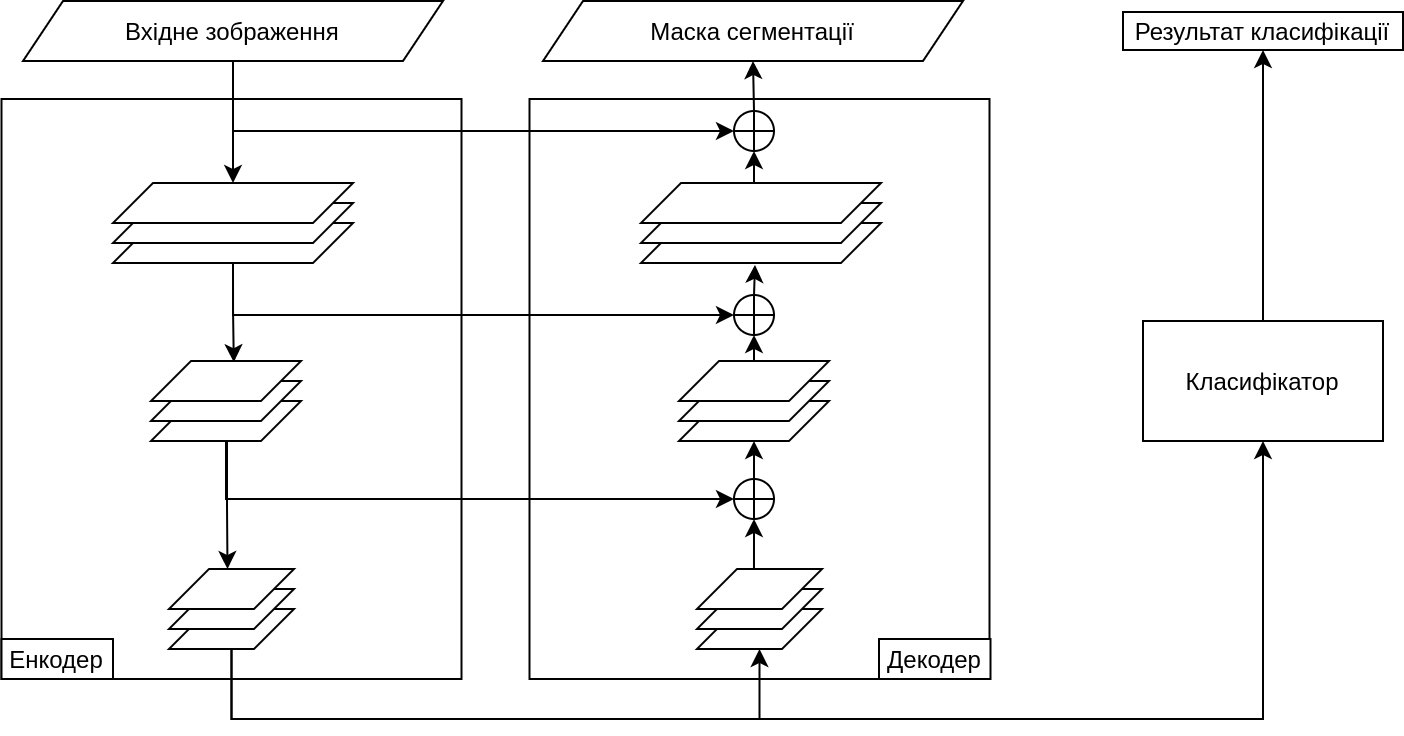
\includegraphics[width=16cm]{my_ne_arch.png}
			\caption{ General neural network architecture with decoder and classifier }
			\label{fig:my_net_arch_intro}
		\end{figure} 
		
		
		Also, the proposed model is presented mathematically. Let the neural network of the encoder be defined as $F_{encoder}$. Then, for the input image $x \in \mathcal{R} ^ {3 \times H \times W}$,  $v_1, v_2, ... v_i, ... v_n$ - a set of sign cards, so $v_i \in \mathcal{R} ^ {c_i \times \frac{H}{i} \times \frac{W}{i}}$, ?? $c_i$ - the number of channels for each of the feature cards, ? $n$ - number of stages encoder (depending on the architecture):
		
		\begin{equation}
			\label{eqn:enc_features_intro}
			v_1, v_2 ... v_n = F_{encoder}(x, \theta_{enc})
		\end{equation}
		
		?? $\theta_{enc}$ - encoder parameter set.
		
		Then, the neural networks of the segmentation and classification decoder can be defined as $F_{seg}$ and $F_{cls}$ accordingly. For a set of feature maps generated by the encoder, we have:
		\begin{align}
			M_{seg} &= F_{seg}((v_1, v_2 ... v_n), \theta_{seg}) \\
			C_{cls} &= F_{cls}((v_n), \theta_{cls})
		\end{align}
		
		where ?????? ?????????? ????????? ??????????? ?? ???????????? ??????????. $\theta_{seg}$ ?? $\theta_{cls}$ - 
		
		The advantage of using the basic LinkNet architecture is the ability to apply transfer training to speed up the training process: the set of encoder parameters $ \ theta_ {enc} $ is initialized using the parameters obtained after training the encoder on the Imagenet data set. The decoder is initialized using the Xe method: $\theta \in \mathcal{U}(-b, b)$, ?? $b$ - ????????? ??????? ??? ???? ????.
		
		Based on the developed neural network model, methods of multitasking learning of deep neural networks and prediction of results are proposed. The method of training neural networks in terms of partially erroneous markup of educational data is based on the use of tasks derived from the original. It is shown that for the problem of semantic segmentation there is a semantically closer more general problem for which the markup of educational data is more accurate than for the original.
		
		Unlike previous methods based on the study of more detailed semantically similar problems, the developed method of using more accurate data for more general problems allows to improve the resolution of internal representations of the neural network, which, in turn, improves the results on the original problem. Also, because the tasks are semantically similar, there is no conflict of gradients, which is typical for learning semantically heterogeneous problems.
		Thus, more general to the problem of semantic segmentation is the problem of classification. In this context, the task of classification is reduced to the task of learning by a set of samples: instead of marking each of the objects for all classes in the image, the image is a bag with one or more objects and appropriate labeling, whether objects of given classes in the image.
		Suppose that for the image  $x \in \mathcal{R}^{3 \times H \times W}$ there is a segmentation mask $y_s \in \mathcal{R}^{C \times H \times W}$ where $C$ - the number of classes, and, $H$ and $W$ the height and width of the image, respectively. If there is at least one marked object of class $?$, in the segmentation mask, the label of the corresponding class $y_c \in (0, 1)^C$ is set in the markup of the classification problem:
		
		
		\begin{equation}
			y_c = t < \sum_{i}^{H} \sum_{j}^{W} y_{s_{ij}}
		\end{equation}
		
		where $t$ - the threshold of the minimum size of the object in pixels
		
		The classification problem generated in this way has a lower probability of erroneous markup.
		
		To reduce the impact of the erroneous part of the markup, a change to the loss function when learning neural networks was proposed for the first time: the loss function for a problem with less accurate markup is limited at the top, so when learning multiple tasks, gradients from incorrect markup do not affect the learning process:
		
		\begin{equation*}
			\mathcal{L} \rceil = min(L, \theta)
		\end{equation*}
		
		where $\theta$ - the threshold limit function loss.
		For the top constraint function, the gradient is defined only on the interval $(-\infty, \theta]$, ?? so for the period $(\theta, \infty)$ gradient is set to zero:
		
		
		\begin{equation*}
			\mathcal{\nabla} min(L, \theta) = 
			\begin{cases}
				1 &\text{$L \in (-\infty, \theta]$}\\
				0 &\text{$L \in (\theta, \infty)$}
			\end{cases}
		\end{equation*}
		
		For each task separately calculated function loss. The top-down loss function is used to train the segmentation decoder, while the classification decoder uses the normal one.
		The total value of the loss function is defined as the arithmetic mean between individual values:
		
		\begin{equation}
			L_{total} = \frac{L_{seg} \rceil + L_{cls}}{2}
		\end{equation}
		
		Accordingly, the total gradient function loss will amount gradients components:
		
		\begin{equation}
			\nabla L_{total} = \frac{\nabla L_{seg} \rceil + \nabla  L_{cls}}{2}
		\end{equation}
		
		The threshold for limiting the loss function for the segmentation problem is a parameter of the learning algorithm and should be chosen empirically depending on the level of errors in the markup. Thus, a gradient "pass" is provided to update the parameters from at least one loss function for each input example.
		
		
		
		Based on the proposed neural network model and the method of its training, a method of combining semantically similar tasks at the forecasting stage has been developed in order to increase the reliability of classification and segmentation of planar images without increasing time.
		????? $C_{cls} \in \mathcal{R}^{C}$ ?? $M_{seg} \in \mathcal{R}^{C \times H \times W}$- Results decoders classification and segmentation, respectively, whose values are in the interval  $(- \infty, + \infty)$ (logites).
		
		For results on the interval $[0, 1]$ using logistic sigmoid activation function:
		$ [0, 1] $ 
		
		\begin{equation*}
			\sigma(x) = \frac{1}{1 + e^{-x}}
		\end{equation*}
		
		The proposed method is to weigh the segmentation map using normalized classifier logs. The first step is the transformation logit segmentation and classification evaluation period due to an uncalibrated $[0, 1]$:
		
		\begin{align*}
			\hat{M}_{seg} &= \sigma(M_{seg}) \\
			\hat{C}_{cls} &= \sigma(C_{cls})	
		\end{align*}
		
		These estimates have the same dimensions as the original mask and classes, for the convenience of representation of operations added additional dimensions to the vector of classes:$\hat{M}_{seg} \in \mathcal{R}^{C \times H \times W}$ ?? $\hat{C}_{cls} \in \mathcal{R}^{C \times 1 \times 1}$ 
		
		The segmentation map is weighed using the Hadamard product between the matrices $\hat{M}_{seg}$ ?? $\hat{C}_{cls}$
		
		\begin{equation*}
			M_{refined} = \hat{M}_{seg} \circ \hat{C}_{cls}
		\end{equation*}
		
		
		
		To improve the ability to interpret model predictions, the method of localization of important image features for classification was improved through the use of multitasking learning methods, which allowed its use in the absence of semantic segmentation markup in the training data set.
		
		The basis of the proposed method is an iterative refinement of the map of localization features by directing the gradients from the classification problem:
		
		The first step is to calculate the refined classification features. To do this, the Hadamard product is calculated between the output of the segmentation decoder normalized by the sigmoid function and the classification logs:
		\begin{equation}
			M_{unsup} = \hat{M}_{seg} \circ C_{cls}
		\end{equation}
		
		Next, to obtain the classification result, the summation of the elements $M_{unsup}$ is performed with normalization by the sum of the elements of the original non-normalized localization map:
		
		\begin{equation}
			C_{unsup} = \frac{\sum_{h=0}^H \sum_{w=0}^{W} M_{unsup(h,w)}}{\sum_{h=0}^H \sum_{w=0}^{W} M_{seg(h,w)} + c}
		\end{equation}
		
		For numerical stability, added to the denominator constant low $c \approx 10^{-5}$
		
		
		Since the scale of the normalized output of the segmentation decoder is in the range $[0,1]$, the use of the Hadamard product allows us to consider $\hat{M}_{seg}$ as a map of the importance of regions for the classification problem. During training the neural network, this structure encourages a combination of tasks neural network to the appointment of high value ($\hat(M)_{seg}\rightarrow 1 $) for important characteristics that are common in images of the training data set.
		where $\sigma(x)$ is a logistic function.
		
		This iterative refinement prompts the neural network to assign high values ($\sigma(M) \rightarrow 1$) to important features that are common in the images from the training data set.
		
		On stage forecasting is used as a classification problem and the problem of localization. Only when the classification output exceeds the specified threshold $T_c$, the localization decoding procedure is performed, otherwise, the localization map is considered equal to zero for all pixels.
		
		Since the outputs of the segmentation decoder $M_{unsup}$ are continuous, and their scale is determined by the learning process, the binarization threshold for localization $T_{seg}$ may be different for different images. To select the optimal threshold $T_{seg}$ on each of the input images, in the post-processing process, it is proposed to use adaptive binarization according to the Otsu method in order to avoid the need to calibrate the neural network predictions.
		
		After performing binarization, mask received over $M_t=M>T_s$ operation performed morphological erosion with a square kernel size 1\% of the image size to get rid of small possible false-positive regions of the mask.
		
		These models and methods were tested in the following subject domains: screening for diabetic retinopathy, screening of steel sheet defects, screening for melanoma, and screening of cloud formations.
		
		
		? \textbf{?????????? ???????}describes the developed tools that implement the proposed methods and tests of the developed method in the framework of experiments on synthetic data generated using the proposed model, as well as experiments in real screening problems. 
		
		The tools are developed in the \textit{Python} programming language using the \textit{PyTorch} automatic differentiation framework. Based on the developed tools, effective software modules have been created, which are integrated with "cloud" services for solving resource-intensive learning tasks of neural networks, which provides high computing power and speed of prediction in automated screening tasks.
		
		Using the model, the proposed methods were tested in different conditions, the analysis of the contribution of individual components was performed and the analysis of the resistance of the proposed method to different levels of marking noise was performed. On average, the increase in the Dyce coefficient relative to the base model was 13\%. For high noise levels, the increase was 42\%.
		
		As part of the \ textit {<< Severstal: Steel Defect Detection >>} project, the proposed neural network models were used on the Kaggle Data Science Competition Platform, and methods were proposed for their training and prediction of results for the problem of semantic segmentation of steel sheet defects. The increase in reliability (Dyce measure) relative to the base model was 4.2\%.
		
		
		As part of the project \textit {<<Understanding Clouds from Satellite Images>>} on the platform for competitions in data science Kaggle used the proposed models of neural networks, as well as methods for training and predicting results for the problem of semantic segmentation of cloud patterns in satellite images. The increase in reliability (Dyce measure) relative to the base model was 3.9\%.
		
		
		As part of the \textit {<<APTOS 2019 Blindness Detection>>} project on the Kaggle Data Science Competition Platform, the proposed methods of multitasking learning and predicting results in the task of classifying fundus photographs for the screening of diabetic retinopathy were used. The increase in reliability (F1-measure) relative to the base model was 2.1\%.
		
		The project \textit{<<SIIM-ISIC Melanoma Classification>>} on the Kaggle Data Science Competition Platform used the proposed localization of classification-relevant image features in the problem of recognizing skin lesions for melanoma screening. The use of the proposed method simplified the process of monitoring the learning of neural networks, which helped prevent retraining and increase the reliability of the classification by 3.5\%.
		
		The methods and tools developed in the work were \textbf {????????????} in the software product SafetyRadar of the company \textit {VITech Lab}, the main purpose of which is to screen the presence of elements of personal protective equipment on people in construction sites, or hospitals and laboratories.
		
\keywords{image analysis, deep neural networks, multitasking machine learning, semantic segmentation, loss functions}
		
\end{abstract}
	
	
	
	%
	%\begin{abstract}[
	%  language=english
	%]
	%  \keywords{}
	%\end{abstract}
